% !TeX spellcheck = en_GB

\chapter{An Adaptive Filter Model of the Cerebellum}
\label{chp:cerebellum}

\vspace{15pt}

\begin{OpeningQuote}
The CNS [Central Nervous System] needs to be understood at four nearly independent levels of description: \emph{(1)} that at which the nature of a computation is expressed; \emph{(2)} that at which the algorithms that implement a computation are characterized; \emph{(3)} that at which an algorithm is committed to particular mechanisms; and \emph{(4)} that at which the mechanisms are realized in hardware.
In general, the nature of a computation is determined by the problem to be solved, the mechanisms that are used depend upon the available hardware, and the particular algorithms chosen depend on the problem and on the available mechanisms.
\OpeningQuoteSource{David Marr and Tomaso Poggio}{From Understanding Computation to Understanding Neural Circuitry (1976)}
\end{OpeningQuote}

\begin{PriorPublication}
This chapter is, with permission from the publisher, in edited and extended from adapted from \citet{stockel2021connecting}.
In turn, this publication is based on work presented at the Cognitive Science Society Conference (\enquote{CogSci}; \cite{stockel2020biologically}) and at the International Conference on Cognitive Modelling (\enquote{ICCM}; \cite{stockel2020connecting}).
\end{PriorPublication}

\begin{Contributions}
The author was responsible for conducting the experiments presented in this chapter, contributing the underlying theoretical work (cf.~previous sections), writing, creating all figures, and conducting the literature review.
Terrence C.~Stewart helped with designing the final network, exploring the parameter space, and writing the paper.
Chris Eliasmith supervised this work and provided helpful feedback.
The novelty of this work lies in demonstrating that we can use the modelling techniques presented above to construct systems that adhere to detailed neurophysiological constraints.
Our results suggest that the Granule-Golgi circuit can, under mild assumptions, generate temporal representations.
Furthermore, by systematically varying neurophysiological parameters in our simulation, we find that the parameters observed in nature tend to be near-optimal for the high-level function we are trying to implement.
\end{Contributions}

\clearpage
% !TeX spellcheck = en_GB

Human cognition is ultimately grounded in neurophysiological processes.
As suggested by Marr's \enquote{levels of analysis} \citep{marr1976understanding}, cognitive scientists tend to implement models of cognition at algorithmic and computational levels, without explicitly taking limitations of the underlying neural substrate into account \citep{eliasmith2015marr}.

Depending on the hypothesis that is being explored, ignoring biological detail can be reasonable. Yet, a closer look at biology may help in two complementary ways.
First, we can \emph{validate} hypotheses about cognition by determining whether it is possible to implement a particular algorithm under the constraints of the biological network in question.  
Second, we can \emph{generate} new hypotheses by asking what class of algorithms a certain network could support.

We believe that cognitive modelling must ultimately embrace a combination of top-down and bottom-up modelling to narrow down the vast space of possible cognitive science theories and to direct research attention within that space.
However, a central roadblock to the adaptation of such methods is the availability of modelling tools that make it possible to specify detailed biological constraints (e.g., neural response curves, spike rates, synaptic time-constants, connectivity patters) while still being abstract enough to facilitate the specification of high-level cognitive function.

One approach designed to help bridge this gap is the Neural Engineering Framework (NEF; \cite{eliasmith2003neural}), in conjunction with the related Semantic Pointer Architecture (SPA; \cite{eliasmith2013how}).
Up until recently however, it has been unclear how to incorporate certain biological constraints that are often described in the neuroscience literature into NEF networks.
For example, and despite initial progress in this direction \cite{parisien2008solving}, accounting for Dale's principle with purely excitatory and inhibitory neuron populations, as well as incorporating spatial connectivity constraints, has been relatively challenging with the existing NEF-based software tool, Nengo \cite{bekolay2014nengo}.
Furthermore, there have been no studies on how adding these additional constraints influences the high-level function of NEF networks. In this paper, we attempt to address both issues.

Specifically, we describe recent advances in modeling techniques that partially alleviate the shortcomings of the NEF mentioned above.
We then use these methods to construct a model of eyeblink conditioning in the cerebellum, with a focus on the generation of temporal basis function representations in the recurrent Granule-Golgi circuit.

Building a model of temporal representation in the cerebellum is of particular interest, since it remains unclear how exactly the cerebellum manages to learn and reproduce the precise timings observed in eyeblink conditioning. Furthermore, the mechanisms underlying eyeblink conditioning are potentially exploited by cognitive processes as well. Recent evidence---ranging from studies in functional connectivity, neuronal tracing, clinical pathology, to evolutionary physiology---suggests that the tasks supported by the cerebellum are not restricted to motor control alone. The cerebellum may instead be recruited by various brain regions as a \enquote{co-processor} to support brain functions related to higher-order cognition, such as language-based thinking, working memory, perceptual prediction, and tasks requiring precise timings in general \citep{sullivan2010cognitive,
           buckner2013cerebellum,
		   oreilly2008cerebellum,
           e2014metaanalysis}.

Our experiments suggest that---at least under the constraints we consider---the Granule-Golgi circuit is well-suited to encode temporal information using basis functions. This representation can be used in the context of a spiking neural network to learn delays by modulating synaptic weights in the granular-to-Purkinje projection.
Furthermore, we generate hypotheses as to why various biological parameters (such as the sparse connectivity patterns and the time-constants of the neurotransmitters) are as observed.

The remainder of this paper is structured as follows.
We first review the high-level function we hypothesize could be implemented in the Granule-Golgi circuit, followed by an overview of the eyeblink conditioning task, the particular neurophysiological constraints of the cerebellum, and high-level theories of cerebellar function.
We then discuss five neural network implementations with an increasing amount of biological detail, along with the corresponding extensions to the NEF.
We perform a series of experiments that explore the impact of individual parameters on the performance of the increasingly realistic system.
We extend our model to perform the complete eyeblink conditioning task by incorporating the remaining cerebellar microcircuitry and compare the model behavior to empirical data.
Finally, we provide a quick overview of \enquote{NengoBio,} the open-source addon to Nengo we developed to encode the aforementioned biological constraints.\footnote{See \url{https://github.com/astoeckel/nengo-bio}.}


\clearpage
\setcounter{subsection}{0}
% !TeX spellcheck = en_GB

\section{Background}

In order to explore the consequences of adding biological details to a neural system, we need to decide---on a computational and algorithmic level---what task the neural system should ideally perform.
As we mentioned above, we would like to implement eyeblink conditioning by mapping an \LTI system generating a sliding-window transformation (cf.~\Cref{sec:temporal_bases}), specifically, the \LDN system, onto the recurrent Granule-Golgi circuit.
We first provide a review of eyeblink conditioning, followed by an overview of the cerebellar microcircuitry thought to be responsible for this behaviour, and, finally, a discussion of hypothesised mechanisms.

\subsection{Eyeblink conditioning}

\begin{figure}
	
\includegraphics{media/chapters/05_cerebellum/conditioning.pdf}
	\caption[Illustration of eyeblink conditioning]{
	Illustration of eyeblink conditioning.
	\textbf{(A)} Before training, the animal shows no reaction to the conditioned stimulus (\CS).
	The animal reacts to the unconditioned stimulus (\US), a puff of air into the eye, with an eyeblink.
	\textbf{(B)} During training, both the \CS and the \US are presented with a fixed delay $\Delta t$.
	\textbf{(C)} After training, the animal reacts to the previously neutral conditioned stimulus with an eyeblink. The delay is maintained; the animal begins to close the eye \emph{before} the puff arrives.
	}
	\label{fig:conditioning}
\end{figure}

Eyeblink conditioning is a form of delay conditioning and a widely studied form of motor learning \citep[e.g.,][Chapter~42, pp.~975-979]{kandel2012principles}.
The overall experimental setup is illustrated in \Cref{fig:conditioning}.
Scientists direct a puff of air, the \emph{unconditioned stimulus} (\US), at the eye of an experimental animal.
This triggers the eyeblink reflex, the \emph{unconditioned response} (\UR).
The animal is then repeatedly exposed to the \US paired with a neutral, \emph{conditioned stimulus} (\CS), for example a short tone.
Here, \enquote{neutral} refers to the fact that the animal typically shows no strong reaction to this stimulus.
The \CS precedes the \US by a constant time offset $\Delta t$.

Over time, the subject forms a \emph{conditioned response} (\CR) to the previously neutral \CS, maintaining the fixed delay $\Delta t$. In other words, the subject will learn to have its eye closed $\Delta t$ seconds after the tone, even if the puff is absent.
In our experiments, we use mouse data from \citet{heiney2014cerebellardependent}.
However, this experiment in principle works in most mammals, including humans \citep{cheng2008neural}.
Importantly, the formation of this conditioned response critically depends on the cerebellum.
Ablating the cerebellum causes previously learned \CRpl to be absent \citep{mccormick1981engram}.
This indicates that the cerebellum is not only capable of establishing the connection between the \CS and the \UR, but also of learning the motor trajectory of the response, including the delay.

\subsection{Cerebellar Microcircuitry}
\label{sec:cerebellum_microcircuit}

\begin{figure}[t]
	\centering
	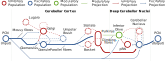
\includegraphics[scale=0.95]{media/chapters/05_cerebellum/cerebellum_anatomy.pdf}
	\caption[Schematic of the cerebellar microcircuit]{Schematic of the cerebellar microcircuit. Dashed projections and populations are not included in our model. Cerebellar nucleus afferents affect both the excitatory and inhibitory sub-populations.  The main feed-forward pathway is highlighted in bold. \emph{\PCN}~$\hat=$~pre-cerebellar nuclei. \emph{pRN}~$\hat=$~parvicellular Red Nucleus. Data from \citet{ito2010cerebellar,llinas2010olivocerebellar}.}
	\vspace*{-0.5em}
	\label{fig:cerebellum_anatomy}
\end{figure}

Before we continue to discuss the two prevalent theories on how the cerebellum could learn the conditioned response, it is worthwhile to review the cerebellar microcircuitry depicted in \Cref{fig:cerebellum_anatomy}.
Afferent nerves from pre-cerebellar nuclei (\PCN; brainstem and cerebral cortex carrying sensory signals) project as \enquote{mossy fibres} onto granule cells in the cerebellar cortex.
Cerebellar granule cells are tiny and account for the majority of neurons in the mammalian brain.
Thus, small numbers of pre-cerebellar neurons connect onto many granule cells.

Granule cells also have interneurons interspersed amongst them, the Golgi cells.
These form an inhibitory feedback loop with the granule cells.
That is, granule cells excite Golgi cells, and Golgi cells inhibit granule cells \citep{ito2010cerebellar}.
Notably, the connections from Golgi and \PCN to granule cells are formed through so-called glomeruli.
Each granule cell extends to on average four glomeruli and, at each glomerulus, receives input from one pre-cerebellar neuron through a mossy fibre terminal, as well as one or more Golgi cells \citep{palkovits1972quantitative,jakab1988quantitative,chadderton2004integration}.
Furthermore, the connectivity between Golgi and granule cells is spatially constrained.
Golgi cells only connect to granule cells within a \SI{600}{\micro\metre} diameter \citep{albus1971theory,dangelo2013cerebellar}.
The ratio of granule to Golgi cells is about $400$:$1$ \citep{korbo1993total}.

Granule cell axons, the so called \enquote{parallel fibres}, project onto the Purkinje cells, which inhibit neurons in the cerebellar nucleus, and in turn project back onto the brainstem and cerebral cortex \citep{ito2010cerebellar,llinas2010olivocerebellar}.
So-called \enquote{climbing fibres} project from Inferior Olive neurons in the deep cerebellar nucleus onto Purkinje cells. 
Evidence suggests that activity in the climbing fibres is responsible for modulating the synaptic strength of granule to Purkinje projections.
Climbing fibre activity is often interpreted as an \enquote{error signal} $\epsilon(t)$ responsible for driving learning in the cerebellar cortex \citep{ito2010cerebellar}.

\subsection{Hypothesised Mechanisms Supporting Delay Learning}

There is no current consensus on what the exact mechanism is that supports delay learning in the cerebellum.
Specifically, there are two competing hypotheses: the classic adaptive filter theory and the view that intrinsic properties of the Purkinje are responsible for timing.
%We review these ideas in more detail below.

\subsubsection{Adaptive filter hypothesis}
As originally pointed out by \citet{marr1969theory,albus1971theory}, the massive divergence (number of post-neurons for a single pre-neuron) and small convergence (number of pre-neurons for a single post-neuron) in the \PCN to granule projection suggests that granular cells are tuned to specific patterns of activity in the \PCN.
Modulating the synaptic weights between the granule and the Purkinje cells using the climbing fibre error signal can be used to recombine the sparse pattern detectors and to decode arbitrary functions.

The adaptive filter hypothesis, originally proposed by \citet{fujita1982adaptive}, can be interpreted as extending this idea toward temporal tuning.
That is, similarly to what we discussed in the previous chapter,
granule cell activity does not only depend on the current \PCN activities, but on their past history.
Correspondingly, if this temporal tuning is diverse enough, that is, granule cells are sensitive to different time-courses, this will form a suitable temporal basis from which functions over time, such as delays, can be decoded.
A possible source for the temporal tuning could be the recurrent granule-to-granule connections that are mediated by the inhibitory Golgi cells.
Indeed, \citet{rossert2015edge} find that randomly connecting the Golgi and granule cells generates diverse tuning that can be exploited as a temporal basis.
Our contribution is to test whether optimal temporal tuning---i.e., an \LTI system approximating a sliding-window transformation (cf.~\Cref{sec:temporal_bases})---could be realised in the Granule-Golgi circuit.


\subsubsection{Intrinsic properties of the Purkinje cells}
A more recent theory is that responses observed in tasks such as eyeblink conditioning inherently rely on intrinsic properties of the Purkinje cells.
In other words, the Purkinje cells act as \enquote{time cells} \citep{lusk2016cerebellar}, and the temporal properties of the granule cells play a lesser role.
Instead, climbing fibre input triggers processes within the Purkinje cell and their dendritic structures that are responsible for the formation of a delayed output.
Evidence for this comes from \citet{johansson2014memory}, who find that bypassing the granule cells and directly injecting signals into the parallel fibres still evokes a previously learned delayed response from the cerebellum, albeit a weaker one.


\subsubsection{Discussion}
We think that these two theories are not inherently contradictory.
Both temporal tuning of the granular cells and intrinsic temporal properties of the Purkinje cells could play a role in delay learning---as we discussed in \Cref{chp:temporal_tuning}, both the intrinsic dynamics of neurons, and the network dynamics can in principle be harnessed to produce desired dynamics.

The findings in this chapter provide a strong argument that the Granule-Golgi circuit is well-suited for implementing some kind of temporal basis, and as such confirms the results of previous studies \citep[cf.][]{dean2010cerebellar,rossert2015edge}.
Still, our work only takes a fraction of the available data on cerebellar neurophysiology into account and as such should not be seen as strong evidence for or against either of the two proposed mechanisms.


\clearpage
\setcounter{subsection}{1}
% !TeX spellcheck = en_GB

\section{Modelling the Granule-Golgi Circuit}
\label{sec:cerebellum_golgi_granule}

As we discussed in the introduction, we would like to analyse in how far adding biological detail to a system influences its high-level function.
To this end, we focus on one specific part of the cerebellar microcircuit, namely the Granule-Golgi circuit, and test to what degree this circuit is capable of generating a temporal representation at five different levels of biological detail.
Below, we first describe these individual circuits, followed by a series of experiments in which we explore the performance of the individual networks.

\subsection{Levels of Biological Detail}
\label{sec:cerebellum_levels}

\begin{figure}
	\centering
	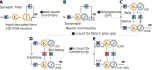
\includegraphics{media/chapters/05_cerebellum/network_types.pdf}%
	{\phantomsubcaption\label{fig:cerebellum_network_types_a}}%
	{\phantomsubcaption\label{fig:cerebellum_network_types_b}}%
	{\phantomsubcaption\label{fig:cerebellum_network_types_c}}%
	{\phantomsubcaption\label{fig:cerebellum_network_types_d}}%
	{\phantomsubcaption\label{fig:cerebellum_network_types_e}}%
	\caption[Network types used in the cerebellum experiments.]{Network types used in our experiments. \textbf{(A)} \enquote{Direct} implementation with an optimal integrator. \textbf{(B)} Using the synaptic filter of a single population of spiking neurons for temporal integration. \textbf{(C)} Inter-neuron population in the recurrent path. \textbf{(D)} Same as \emph{(C)}, but accounting for Dale's principle. \textbf{(E)} Same as \emph{(D)}, but with more detailed biological constraints (see text).}
	\label{fig:cerebellum_network_types}
\end{figure}

We discuss five models of increasing complexity (cf.~\Cref{fig:cerebellum_network_types}).
The first model is merely an abstract implementation of the delay network, the final model respects spatial connectivity constraints, tuning curves, and, to a degree, neurotransmitter time-constants.
In all cases, the input $u$ is received from an \NEF ensemble with $100$ spiking \LIF neurons representing the \PCN.

\subsubsection{Model A: \enquote{Direct} Implementation} 
For this model, we directly solve the differential equations describing the Legendre system (cf.~eq.~\ref{eqn:delay_network_lti}) by integration.
% TODO: Add correct reference to the delay network
That is, we have a single layer of \enquote{neurons} that are pure integrators.
Correspondingly, this model focuses on the high-level theory of what the system is computing.
We model the \PCN and the granule cells as neuron populations, but these are not responsible for generating the dynamics.

\subsubsection{Model B: Single Population}
In our second stage, we replace the integrators with an ensemble of $200$ \LIF neurons.
As we discussed in \Cref{sec:nef_representation}, these neurons form a distributed representation of the Legendre system state $\vec{m}$ using a population code (cf.~eq.~\ref{eqn:encoding}).
Maximum firing rates $a_\mathrm{max}$ are between \SIrange{50}{100}{\hertz}.
We solve for optimal input and recurrent connection weights that result in these desired tuning curves while implementing the equivalent calculation as in \emph{Model A} using the \NEF dynamics principle (\Cref{sec:nef_dynamics}).

\subsubsection{Model C: Inter-neurons}
As a next step, we separate the single layer of neurons into two populations corresponding to the Golgi and granule cells, reflecting the actual biology of the cerebellum.
This introduces two synaptic filters which need to be taken into account when solving for the connection weights that best approximate the Legendre system; we discussed this in \Cref{sec:lti_complex_networks}.
Furthermore, to at least approximate the fact that there are far fewer Golgi cells than granule cells, we use $20$ Golgi cells and $200$ granule cells.

\subsubsection{Model D: Inhibition and Excitation}
In the next step, we account for Dale's principle using the techniques described in \Cref{sec:nef_nonneg}.
We mark the graunle cells as purely excitatory, and the Golgi cells as purely inhibitory and decode the bias current from the pre-population.
Note that we assume---in contrast to the evidence presented in \Cref{fig:granule_jbias_distribution}---that the granule cells possess intrinsic biases and uniform $x$-intercepts; we discuss this in more detail below.

\subsubsection{Model E: Sparse connectivity and activities}
Finally, we constrain the neural connectivity and adjust the \PCN tuning.
The previous models used all-to-all connections, whereas we now only allow a subset of the connection weights to be non-zero.
This applies to both the input to the Granule-Golgi system and to the recurrent connections.

In particular, as is indicated in \Cref{fig:cerebellum_network_types_e}, we account for the granule cell convergence numbers by randomly selecting five \PCN and five Golgi cells as pre-neurons---this number is slightly larger than the number reported above, since, as we discuss in more detail in \Cref{sec:cerebellum_vary_parameters}, the number of pre-neurons places a strict upper limit on the connectivity. Given this extremely sparse connectivity, we increase the number of neurons in the simulation to \num{10000} granule and \num{100} Golgi cells, which is closer to the ratio observed in nature.

\begin{figure}
    \centering
    \includegraphics{media/chapters/05_cerebellum/spatial_constraints.pdf}
    \caption[Spatial connectivity constraints between the Golgi and granule cells]{Spatial connectivity constraints between the Golgi and granule cells.
    \textbf{(A)} Normalised connection probabilities $p_{ij}$ for $\sigma=0.25$. Note that the neuron locations are sampled from a Hilbert curve with additive random jitter. Correspondingly, neurons with similar (relative) indices tend to be closer together, resulting in the clearly visible diagonal.
    \textbf{(B)} Spatial organisation of the Golgi and granule cells. The background depicts the cumulative density of the Golgi to granule connection probability for a virtual Granule cell at each location; same colours as in \emph{(A)}.}
    \label{fig:spatial_constraints}
\end{figure}

\begin{figure}
	\centering
    \includegraphics{media/chapters/05_cerebellum/pcn_tuning.pdf}
    \caption[Granule cell EPSC distributions and PCN tuning curves]{Granule cell \EPSC distributions and \PCN tuning curves.
    \textbf{(A)} Empirical granule cell \EPSC rates (cf.~\cite{chadderton2004integration}, Figure 3C; rescaled from counts per bin to rates).
    Data are the mean over 16 trials.
    Black bar and shaded background correspond to stimulation of the animal's whiskers.
    Upper dashed line corresponds to the average spike rate with input (including the first bin after the input), lower dashed line to the average spike rate without input.
    \textbf{(B, C)} In our model, \PCN input via the mossy fibres is the only excitatory input to the granule cells. Setting the maximum firing rates to be uniformly distributed in $[25, 75]$ and the $x$-intercepts to be uniformly sampled from $(-0.15, 0.95)$ qualitatively results in a similar \EPSC distribution. Data are the mean over \num{10000} cells.
    }
    \label{fig:pcn_tuning}
\end{figure}

To account for spatially imposed connectivity constraints, we assign a location $\vec x$ in $[-1, 1]^2$ to each neuron.
This represents to a location on a small patch of the folded two-dimensional surface of the cerebellar cortex.
As is depicted in \Cref{fig:spatial_constraints}, the probability $p_{ij}$ of a post-neuron $i$ to receive a connection from a pre-neuron $j$ is proportional to $\exp \left(- \| \vec x_i - \vec x_j \|^2 / \sigma^{2} \right)$.%
\footnote{See \Cref{sec:nengo_bio_sparsity} for an overview of how these sparsity constraints can be specified in NengoBio.}

The input representation in the \PCN was made more temporally sparse by adjusting the $x$-intercepts (\Cref{sec:nef_representation}).
Data reported by \citet{chadderton2004integration} indicate that granule cell excitatory event rates---which are driven by \PCN activity---drop from an average of \SI{40}{\per\second} with a stimulus being present to only \SI{8.5}{\per\second} when there is no stimulus.
We adjusted the \PCN tuning curves to match these statistics in the final network (cf.~\Cref{fig:pcn_tuning}).


\subsection{Impact Of Biological Detail On Temporal Representations}

To explore the effect of adding biological detail to the Granule-Golgi circuit, we first take a look at the temporal representations generated by these systems.
We then analyse in how far we are able to decode delays from these representations, as is required for delay conditioning.

\subsubsection{Temporal Representations}

\begin{figure}
	\centering
    \includegraphics{media/chapters/05_cerebellum/basis_functions.pdf}%
    {\phantomsubcaption\label{fig:cerebellum_basis_functions_a}}%
    {\phantomsubcaption\label{fig:cerebellum_basis_functions_b}}%
    {\phantomsubcaption\label{fig:cerebellum_basis_functions_c}}%
    {\phantomsubcaption\label{fig:cerebellum_basis_functions_d}}%
    {\phantomsubcaption\label{fig:cerebellum_basis_functions_e}}%
    {\phantomsubcaption\label{fig:cerebellum_basis_functions_f}}%
    {\phantomsubcaption\label{fig:cerebellum_basis_functions_g}}%
    \vspace{0.5em}
    \caption[Temporal response of the Granule-Golgi networks]{
    	Temporal response of the Granule-Golgi networks for a rectangle input (black line).
    	All responses are centred and normalised.
    	\emph{Left:} Example identity decoding of the granule activities.
    	\emph{Centre and right:} Example singular value decomposition (\SVD) of the granule cell activities and the median normalised singular values over \num{100} trials. Error-bars indicate the 25th and 75th percentile.
    	\textbf{(A-E)} Data for the individual models discussed in this section.
    	\textbf{(F)} Network with a stable random feedback matrix~$\mat A$.
    	\textbf{(G)}~Disabling intrinsic biases substantially reduces the performance of the network.
    }
    \label{fig:cerebellum_basis_functions}
\end{figure}

\Cref{fig:cerebellum_basis_functions} depicts the response of the different Granule-Golgi circuits for a rectangle input.
When decoding $\vec{\hat m}$ using the identity decoder (eq.~\ref{eqn:lstsq_loss_identity}), we find that adding detail increases the amount of noise and decreases the similarity with the \enquote{direct} implementation.
The decoding for the most detailed network, \emph{Model E}, is less noisy due to the large number of granule cells, but does not resemble the direct implementation at all.

However, the fact that $\vec{\hat m}$ is not close to the desired $\vec m$ does not imply that the granule cell \emph{activities} do not form a useful temporal representation.
A singular value decomposition of the filtered granule cell activities reveals that the realistic network establishes a temporal representation that resembles the Legendre basis and---judging from the norm of the singular values---is almost as expressive as that of the unconstrained two-population model.
A control experiment (\Cref{fig:cerebellum_basis_functions_f}) with random stable feedback matrices $\mat A$ demonstrates that solving for the Legendre system is significantly better than solving for 

Interestingly, deactivating intrinsic biases in the granule cells (\Cref{fig:cerebellum_basis_functions_g}) leads to a substantial decrease in the quality of the generated representation.
This implies that if the granule cells indeed form a temporal representation in nature, then granule cell tuning must be diversified using a mechanism that is not captured by our model.

\subsubsection{Decoding delays}

\begin{figure}
	\centering
	\includegraphics{media/chapters/05_cerebellum/2d_sweeps.pdf}
	\caption[Delayed signal reconstruction errors in the Cerebellum model.]{Delayed signal reconstruction error for different types of input signals, delays, and network types. All error values are expressed as \RMSE divided by the mean \RMS of the input signal over 100 trials. Columns correspond to the network types in \Cref{fig:cerebellum_network_types}. \emph{Top row:} Reconstruction error for rectangle pulse signals of varying width. \emph{Bottom row:} Reconstruction error for a band-limited white noise input signal with varying band-limit.}
	\label{fig:cerebellum_2d_sweeps}
\end{figure}

\begin{figure}
	\centering
    \includegraphics{media/chapters/05_cerebellum/delay_example.pdf}%
    {\phantomsubcaption\label{fig:delay_example_a}}%
    {\phantomsubcaption¸\label{fig:delay_example_b}}%
	\caption[Examples showing the delayed input signals decoded form the granule layer in the detailed model.]{Examples showing the delayed input signals decoded form the granule layer in the detailed model (\Cref{fig:cerebellum_network_types_e}). \emph{Top row:} Input signal (rectangle pulses in \textbf{A}, white noise in \textbf{B}). \emph{Middle row:} Spike raster for 40 randomly selected granule cells. \emph{Bottom row:} Delays decoded from one thousand randomly selected granule cells. Dotted lines correspond to an optimal delay.}
	\label{fig:cerebellum_delay_example}
\end{figure}

To test in how far the temporal representations generated by the Granule-Golgi network can actually be used to decode delayed versions of an input signal, we systematically generate two different types of input $u(t)$: periodic pulses of varying width $t_\mathrm{on}$ and band-limited white noise of bandwidth $B$.
%These are meant to represent inputs that may arise in experimental (pulses) and real-world situations (white noise).
We then determine how accurately the past history $u(t - \theta')$ over the window $\theta = \SI{0.4}{\second}$ can be recovered from the granule activity via optimal linear readout weights.
We simulate the network for $T = \SI{10}{\second}$.

\Cref{fig:cerebellum_2d_sweeps} depicts the average reconstruction error for varying inputs (horizontal axis) and delays (vertical axis) over ten trials.
An example run of \emph{Model E} (the model with the most biological detail) is shown in \Cref{fig:cerebellum_delay_example}.
%The different decoded output lines (bottom) are all based on the same neural activity (middle), but with different readout weights.
Overall, the network successfully functions as a method for encoding the input signal over the desired window of time $\theta$.
As predicted by the previous experiment, adding more biological detail generally decreases the accuracy of the system, and \emph{Model E} outperforms \emph{Model D}.
Note that there is a peak in accuracy when decoding data from $\theta' = \SI{60}{\milli\second}$ in the past ($\theta'/\theta=0.15$).
This corresponds to the neurotransmitter time-constant $\tau = \SI{60}{\milli\second}$ we use for all connections in the Granule-Golgi circuit, and which is based on a first-order low-pass fit to the NMDA Granule-Golgi dynamics reported in \citet{dieudonne1998submillisecond}.%
\footnote{Note that the reported time-constants of other connections in the Granule-Golgi circuit are significantly shorter \citep{kanichay2008synaptic}.
While we could use the techniques from the previous chapter to compute the connections weights for these heterogeneous $\tau$, we assume homogeneous $\tau$ for the sake of simplicity.}

\clearpage

\subsection{Parameter Exploration}
\label{sec:cerebellum_vary_parameters}

\begin{figure}[t]%
	\centering
	\includegraphics{media/chapters/05_cerebellum/parameter_sweeps.pdf}%
	\includegraphics{media/chapters/05_cerebellum/convergence_histogram.pdf}%
	{\phantomsubcaption\label{fig:cerebellum_param_sweeps_a}}%
	{\phantomsubcaption\label{fig:cerebellum_param_sweeps_b}}%
	{\phantomsubcaption\label{fig:cerebellum_param_sweeps_c}}%
	{\phantomsubcaption\label{fig:cerebellum_param_sweeps_d}}%
	\caption[Cerebellum model parameter exploration.]{Parameter exploration. \textbf{(A-C)} Effects of varying parameters on the delay reconstruction error (arrows indicate default parameters). The box plots show the median, lower and upper quartile of all the data depicted a single plot in \Cref{fig:cerebellum_2d_sweeps} ($n = 441$ data points). \textbf{(D)} Histograms showing the frequency of measured \PCN to granule convergences compared to the desired convergences.}
	\label{fig:cerebellum_param_sweeps}
\end{figure}

Notably, we can use our model to determine what the accuracy would be like if we changed individual parameters, such as the aforementioned synaptic time-constant.
This is shown in \Cref{fig:cerebellum_param_sweeps}.
Interestingly, the performance of the system is best for a filter time-constant of \SI{50}{\milli\second}, which is closed to the value we used based on measured Granule-Golgi dynamics.

As discussed above, a striking feature of the cerebellar microcircuitry is the low granule cell convergence. One possible hypothesis is that these numbers are a trade-off between minimising connectivity and the overall performance of the resulting system.
In our model, we can test this hypothesis by systematically varying the number of pre-neurons the solver has access to. Results are shown in \Cref{fig:cerebellum_param_sweeps_b,fig:cerebellum_param_sweeps_c}.

For the \PCN to Granule convergence (\Cref{fig:cerebellum_param_sweeps_d}), the performance of the system does improve with larger limits, yet plateaus at still relatively small convergence numbers.
Importantly, as mentioned above, the desired convergence solely controls the number of \emph{potential} pre-neurons.
Since the weight solver may still set a weight to zero, these convergence numbers are upper limits.
Measuring the actual convergence in the \PCN to granule connections (\Cref{fig:cerebellum_param_sweeps_d}), we see a peak at one to three \PCN cells connecting to each granule cell, and this peak is only weakly affected by the desired convergence.
Importantly, in nature, \PCN cells connect to on average four granule cells (see \cite{palkovits1972quantitative}, for the complete statistics), whereas we only measure an average convergence of two in our model (for a desired convergence of five).
We can match the observed average in our model by increasing the desired convergence to $13$.
This slightly increases the performance of the system and coincides with the optimal desired convergence (cf.~\Cref{fig:cerebellum_param_sweeps_b}).
Nevertheless, since the gain in performance is relatively small, we decided not to alter the desired convergence in our model setup.

\Cref{fig:cerebellum_param_sweeps_c} indicates that the performance of the system improves up to a desired Golgi to granule convergence number of $13$, with a measured average convergence of $4.8$ in the final network.
This is a little higher than what is commonly assumed in the neuroscience literature, although, notably, there is some uncertainty regarding this number.
The original study by \citet{jakab1988quantitative} on the physiology of individual glomeruli (the sites receiving Golgi cell axons and granule cell dendrites; cf.~\Cref{fig:cerebellum_anatomy}) counts up to $145$ Golgi axon synapses in one glomerulus.
However, it is unclear whether these synapses originate from a single or different Golgi cells.
Most researchers assume at most one Golgi cell connecting to each glomerulus, and, as explained above, each granule cell in turn connecting to on average of four glomeruli \citep{palkovits1972quantitative}.
Our model predicts that if the Granule-Golgi circuit were to generate a temporal representation, then multiple Golgi cells sometimes connect to the same glomerulus.



\setcounter{subsection}{2}
% !TeX spellcheck = en_GB

\section{Extension Toward a Model of Eyeblink Conditioning}

Given the above model for the Golgi and granule cells, we can now introduce learning into the model to test the behavior of the system in an eyeblink conditioning task.
Since we are mostly interested in whether it is possible at all to decode functions online from the Granule cell activities, we do not focus on biological detail for the added components beyond the standard NEF techniques discussed in \Cref{sec:nef}.
For example, we do not account for Dale's principle for the added neuron populations and use relatively few spiking neurons at high maximum firing rates (\SIrange{200}{400}{\per\second}) to represent individual ensembles.

\subsubsection{Network description and learning}
Our final network architecture is depicted in \Cref{fig:eyeblink_network}.
Consistent with the adaptive-filter hypothesis of cerebellar function and as discussed in \Cref{sec:cerebellum_microcircuit}, we assume that the error signal $\varepsilon(t)$ originates from the Inferior Olive (IO).
This signal is the difference between the conditioned response (what the model has learned so far), and the unconditioned response (the motor response produced by the innate eyeblink reflex).
We model the eyelid as a first-order dynamical system that receives a velocity command.
The reflexive velocity command has been fitted to the UR data in \citet{heiney2014cerebellardependent}.

\begin{figure}
	\centering%
	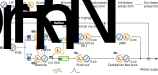
\includegraphics{media/chapters/05_cerebellum/eyeblink_network.pdf}
	\caption[Overview of the final eyeblink conditioning network]{Overview of the final eyeblink conditioning network. Note that our model of the Purkinje cells and the deep cerebellar nuclei is less biologically detailed than the Granule-Golgi circuit.
	}
	\label{fig:eyeblink_network}
\end{figure}

To adjust the connection weights between the granule cells and the Purkinje cells, we use the Prescribed Error Sensitivity (PES) rule defined by \citet{macneil2011finetuning}, a biologically plausible variant of the classic delta learning rule.
Let $w^{\mathrm{Gr}\to\mathrm{Pu}}_{ij}$ be the connection weight between the $j$th granule cell and the $i$th Purkinje cell, $\eta$ a learning rate parameter, $a^\mathrm{Gr}_j(t)$ the $j$th post-synaptic granule cell activity filtered by a low-pass filter with time-constant $\tau_\mathrm{learn}$, and $e^\mathrm{Pu}_i \in \{-1, 1\}$ the encoder of the $i$th Purkinje cell.
The PES learning rule is given as
\begin{align*}
	\frac{\partial}{\partial t} w^{\mathrm{Gr}\to\mathrm{Pu}}_{ij}(t) &= -\eta \varepsilon(t) e^\mathrm{Pu}_i a^\mathrm{Gr}_j(t) = -\eta \sum_{k} w^{\mathrm{IO}\to\mathrm{Pu}}_{ik} a^\mathrm{IO}_k(t) \,,
\end{align*}
where $a^\mathrm{IO}_k(t)$ is the activity of the $k$th IO cell, and $w^{\mathrm{IO}\to\mathrm{Pu}}_{ik}$ are the synaptic weights between the $k$th IO cell and the $i$th Purkinje cell.
These weights are the product of the Purkinje cell encoder $e_i^\mathrm{Pu}$ and a decoding vector $\vec d_k^\mathrm{IO}$ that linearly decodes the error signal $\varepsilon(t)$ from IO cell activity.

Most parameters were set based on biological data; the synaptic time-constant $\tau = \SI{5}{\milli\second}$ except in the Granule-Golgi microcircuit, as described above.
The only free parameters are the learning rate $\eta=180\times 10^{-6}$, $\tau_\mathrm{pRN} = \SI{100}{\milli\second}$ for the connections involving the pRN, and $\tau_\mathrm{learn} = \SI{60}{\milli\second}$ for filtering the granule cell activity in the learning rule.
The learning rate was adjusted to match the number of trials typically needed for mice to learn the task ($\approx 300$ trials).
Velocity commands smaller than $v_\mathrm{th} = \SI{2}{\milli\metre\per\second}$ are counted as zero.

\begin{figure}
	\centering%
	\includegraphics{media/chapters/05_cerebellum/blink_trials_panel.pdf}
	\caption[Model and experimental data for the eyeblink conditioning task]{Model and experimental data for the eyeblink conditioning task. \textbf{(A, B)} Maximum CR triggered eyelid closure over $500$ trials for six random instances of the model/experimental animals. Gray dots correspond to the eyelid closure at the time of the US. Black line is the moving average over 11 trials. Blue dotted lines correspond to an experimental day, that is, $100$ trials in simulation, and up to $100$ trials in the animal experiment. \textbf{(C, D)} Eyelid closure trajectory averaged over one experimental day and all six models/animals. \textbf{(E)} Eyelid velocity signal decoded at the Purkinje cells compared to the reflex-triggered velocity signal. Data for \textbf{(B, D)} adapted from \protect\citet{heiney2014cerebellardependent}.}
	\label{fig:result-basic}
\end{figure}

\subsubsection{Results}
\Cref{fig:result-basic} shows the behaviour of a typical run of the detailed version of our model performing the eyeblink conditioning task over 500 trials.
The \enquote{tone} (CS) is modeled as a rectangle pulse with $t_\mathrm{on} = \SI{100}{\milli\second}$.
The \enquote{puff} (US) occurs \SI{250}{\milli\second} after the CS onset.
The model learns to have the eye closed when the puff occurs. Notably, individual instances of the network show slight differences in learning speed, just as individual experimental animals do.

While our model reproduces key features of eyeblink conditioning, its behavior differs from the experimental data in some aspects.
Foremost, the model does not reproduce the increase in learning speed over time; to the contrary, learning slows down as the model converges to the optimal set of parameters.
Furthermore, our model shows far less inter-trial variance compared to experimental animals.
We think that the reasons for this are twofold.
First, the $10\,000$ granule cells used in our experiments provide an on average very stable temporal basis from which we can decode the motor control signal.
Second, we do not model external systems that might interfere with the cerebellar motor commands, such as signals originating from motor cortex, or the physics of the eyelid itself.
Since these processes may be a significant source of inter-trial variance, it is not unsurprising that our model produces a relatively noise-free output.
Still, more research in these areas will be required in the future.


\subsubsection{Discussion of the synaptic filter $\tau_\mathrm{learn}$}
The low-pass filter $\tau_\mathrm{learn}$ on the learning connection can be interpreted as summarising temporal filtering corresponding to the mechanisms driving synaptic plasticity \citep[e.g.,][Chapter~66]{kandel2012principles}.
Functionally, $\tau_\mathrm{learn}$ is required to reproduce the observation that the animal will close the eye \emph{before} the puff occurs as learning progresses.
Without the filter, the system learns to close the eye soon \emph{after} the puff; our system tries to exactly re-create the motor pattern produced by the unconditioned reflex---which closes the eye \emph{after} the puff happens.

However, by slowing the passage of information from the Cerebellar Nucleus back to the IO, we are effectively comparing the reflex at one point in time to the generated output from the cerebellum at an \emph{earlier} point in time.
This allows the new learned reflex to occur slightly earlier than the unconditioned response, and thus the eye closes before the air puff.
We note that this is a situation where adding biological detail (the synaptic filtering) improves the performance of the model.
If the model were to learn to \textit{exactly} reproduce the UR given the CS, then the eyeblink would occur \textit{after} the puff of air, which would be a less useful response.

\clearpage
\setcounter{subsection}{3}
% !TeX spellcheck = en_GB

\section{Discussion}

We mapped a high-level, mathematical function onto a brain microcircuit while incorporating biological constraints.
Although we were not able to precisely fit the desired Legendre system onto the most detailed Granule-Golgi circuit, the resulting system implicitly produces a good temporal representation, and the quality of this representation critically depends on trying to implement the Legendre system.

The key difference of our approach to existing models of the Granule-Golgi circuit (such as \cite{rossert2015edge}) is that our modelling techniques are more general with respect to the high-level function that is being mapped onto the underlying circuit.
Instead of relying on random connectivity, we specify the high-level function we would like the system to perform.

\subsubsection{Predictions}
We demonstrated that measurements from our model can be used to generate hypotheses about the kind of electrophysiological data we would expect to find, if this function was indeed realised in the brain.
Having access to low-level biological parameters \emph{in silico} furthermore facilitates the exploration of physiological changes that are difficult to achieve experimentally \emph{in vivo}.
As discussed above with respect to the synaptic time-constants and convergence numbers, this allows us to investigate why certain parameters are as observed.
Furthermore, directly tying the time constant to the behavioural performance suggests what kind of behavioural effects would be observed if we could shorten the time constant \emph{in vivo}.

Importantly, our results indicate that the Granule-Golgi circuit could in principle implement a temporal basis function representation.
However, as we discussed above, this is under the condition that the Granule cell response curves are diversified by some mechanism not directly captured by our model.
Without diverse granule tuning curves the expressiveness of the generated temporal representation is reduced, although not fully unusable.
We furthermore predicted that the Granule-Golgi circuit would be better suited for temporal basis function generation if more than one Golgi cell would sometimes connect to a glomerulus.

\subsubsection{Future work}
While our model of eyeblink conditioning is concerned with a relatively low-level task, the techniques presented here for mapping function onto brain microcircuits are applicable to models of higher-level cognitive function as well, beyond what was already possible with the \NEF and Nengo.
In particular, it would be interesting to see whether our model of the Granule-Golgi circuit in conjunction with the Purkinje cell's plasticity could serve as a supervised learner for timings in cognitive and perceptual tasks, as suggested by various studies \citep{oreilly2008cerebellum,e2014metaanalysis,sanger2020expansion}.

Future work should focus on incorporating additional biological detail into the model (such as separate biological time-constants for all synapses); specifically, it would be interesting to extend the detail applied to the Granule-Golgi circuit to the remaining portions of the cerebellar microcircuit.
Furthermore, it would be interesting to find potential mechanisms for the diversification of the Granule cell tuning curves and to gain a better understanding of why the Legendre system cannot be mapped exactly onto the detailed Granule-Golgi circuit.
